\documentclass[a4paper,12pt,titlepage,italian,openany]{report}

\usepackage[font=footnotesize,labelfont=bf]{caption}
\usepackage{babel}
\usepackage{url}
\usepackage{frontespizio}
\usepackage[utf8]{inputenc}
\usepackage{graphicx}
\usepackage{epstopdf}
\usepackage{geometry}
\usepackage[document]{ragged2e}
\usepackage[babel]{csquotes}
\usepackage[hidelinks]{hyperref}
\usepackage{tocbibind}
\usepackage{float}


\linespread{1.2}
\begin{document}
\epstopdfsetup{outdir=./}
\begin{frontespizio}
\Universita{Pisa}
\Facolta{Dipartimento Di Informatica}
\Corso[Laurea]{Informatica}
\Logo{pisalogo}
\Titoletto{Relazione Finale}
\Titolo{Implementazione di un sistema di tracing\\
per architetture a micro servizi}
\Candidato[559556]{James Luigi Francario}
\Relatore{Prof. Daniele Mazzei}
\Relatore{Giacomo Baldi}
\Relatore{Davide Neri}
\Annoaccademico{2019-2020}
\end{frontespizio}

\tableofcontents

\chapter{Introduzione}
\section{}
Il tirocinio si è  svolto presso l' azienda Zerynth con sede a Pisa , Largo Padre Renzo Spadoni 1.
La durata del tirocinio è stata di circa due mesi, per un totale di circa 300 ore di lavoro.
\\
L' obiettivo è stato quello di sviluppare un sistema di tracing dei micro servizi dello ZDM\cite{zdm:1} (Zerynth Device Manager), ovvero
l' applicazione distribuita dell' azienda. Quest' applicazione permette agli utenti di gestire tutti i dispositivi che fanno parte di una rete del tipo
Internet of Things (IoT).\\
L' architettura del sistema \`e a micro servizi, dunque è formato da molti servizi di piccole dimensioni che comunicano tra loro attraverso richieste HTTP oppure,
come vedremo in seguito, con uno scambio di messaggi. 

\section{}
Il sistema di tracing \`e stato sviluppato da zero, ovvero non c'è stata alcuna base di partenza. Il lavoro è stato svolto in parziale autonomia,
da casa, interrotto da qualche riunione svolta in ufficio per chiarire dubbi, tenere traccia del lavoro svolto e per partecipare alle riunioni del team di sviluppo dello ZDM\cite{zdm:1}.\\
Il lavoro è stato seguito dal responsabile dello sviluppo software Davide Neri, con il quale si è tenuta una costante comunicazione per discutere del lavoro svolto e dei nuovi compiti da fare.

\section{Organizzazione Relazione}
La relazione proseguirà in questo modo:
\begin{itemize}
    \item Un breve capitolo che espone le basi di partenza
    \item Un capitolo sull' architettura finale del sistema
    \item Un capitolo sulle tecnologie utilizzate e perché sono state utilizzate, con una spiegazione piú o meno dettagliata di ogni tecnologia
    \item Un capitolo sul lavoro svolto 
    \item Un capitolo di conclusione, dove si andrà a tirare le somme del tirocinio e discutere se si è ottenuto o meno l' obiettivo del tirocinio.
\end{itemize}



\chapter{Basi di Partenza}
\section{Scelta del tirocinio}
Innanzitutto diamo motivazione della scelta di svolgere un tirocinio anziché una classica tesi triennale.In primo luogo è semplicemente perché le idee di un possibile argomento
per una tesi scarseggiavano; ma il motivo principale è che l' autore cercava qualche progetto pratico che lo potesse introdurre in un ambiente lavorativo, per affinare le sue abilità pratiche. Dunque l' autore ha iniziato a cercare tra i vari tirocini proposti nell' apposito albo. Non soddisfatto delle varie proposte, e notato che quasi tutti fosserò già occupati, si è preferito chiedere direttamente al Professore Daniele Mazzei, il quale nelle lezioni del corso di Programmazione di Interfacce ha introdotto agli studenti l'azienda di Zerynth della quale è co-fondatore; ha invitato a lezione 
il CTO dell' azienda Giacomo Baldi per discutere del lavoro svolto da Zerynth ed di eventuali occasioni di tirocini. Dunque l'autore ha scritto al professore per dichiarare il suo interesse per un eventuale tirocinio, e dopo un breve colloquio con G.Baldi è stato proposto questo tirocinio sullo sviluppo di un sistema di tracing per architettura a micro servizi.
\section{Preparazione autonoma}
Dopo essermi incontrato con i miei tutori aziendali, ci siamo accordati su cosa studiare autonomamente per prepararsi allo sviluppo del sistema.
Prima di tutto, ci si è focalizzato  sullo studio autonomo del linguaggio di programmazione Golang poiché è il linguaggio utilizzato per lo ZDM\cite{zdm:1}.
Poi si è proseguito con lo studio delle librerie di opentracing, una libreria open-source che permette di tracciare micro servizi.
Questo studio è stato effettuato tramite un tutorial\cite{opentracing:2} messo a disposizione da uno degli sviluppatori della libreria. Dopo di che, per avere un' idea piú chiara su come funzioni lo ZDM,
ho studiato autonomamente la libreria di Go kit\cite{go:2}, una libreria di Golang che permette una facilitata gestione dei micro servizi.
Assieme ad opentracing si è anche studiato le librerie di Jaeger\cite{jaeger:1}, uno strumento che serve in parallelo con opentracing.
Le tecnologie menzionate verranno approfondite nel capitolo seguente.
\chapter{Tecnologie utilizzate}
\section{Golang}
Golang\cite{go:1} è il linguaggio utilizzato per lo sviluppo dello ZDM. Dato che questo sistema di tracing va instrumentato nel codice dell'applicazione, si è dovuto per forza utilizzare le librerie
Golang di opentracing (sono disponibili in diversi linguaggi).
\section{Opentracing}
Opentracing\cite{opentracing:1} è il cuore di questo progetto. È una libreria open-source sviluppata per il tracing dei micro servizi facenti parti di un' applicazione.
Quello che permette di fare è di tracciare le chiamate e le operazioni dei micro servizi in modo facile e immediato.
Questo lo fa attraverso due oggetti: Gli \textbf{span} e i \textbf{trace}.\\
\subsection{Span}
Sono degli oggetti che rappresentano una singola operazione di un micro servizio. Ogni span ha un proprio ID, una durata, 
gli si possono aggiungere dei tag che sono coppie chiave valore, oppure dei log, messaggi che contengono informazioni. Un tipo speciale di log è il LogError che permette
di evidenziare gli errori in cui un micro servizio va incontro. Un' altro oggetto che può essere associato ad uno span è il baggageItem, ovvero un qualunque tipo di oggetto a cui può accedere chiunque abbia un riferimento a quello span.
\subsection{Trace}
Un trace è una sequenza di span in relazione tra loro, possono essere dello stesso servizio oppure appartenere a servizi diversi. Anche i trace hanno un ID e una durata.
Nella figura 3.1 possiamo vedere un' idea concettuale di come questi due oggetti sono in relazione.

\begin{figure}[H]
    
    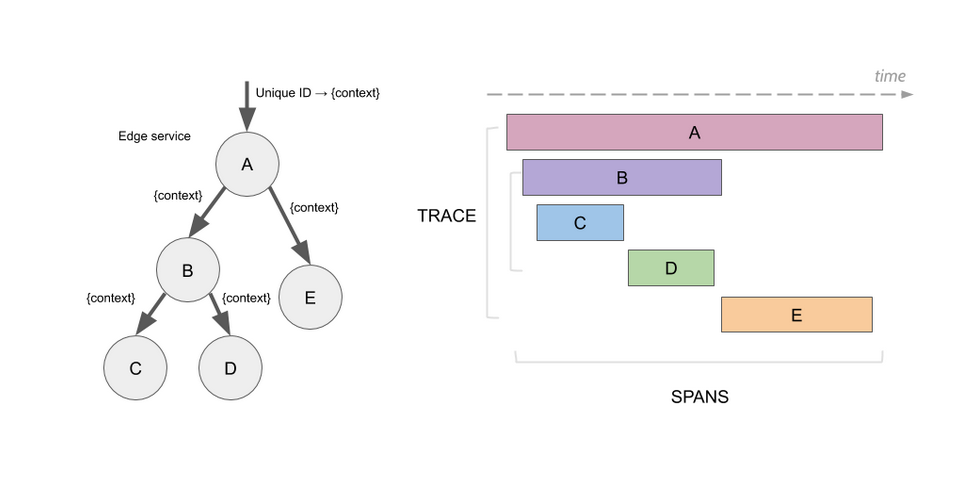
\includegraphics[scale=0.4]{1.png}
    \centering
    \caption{Colori diversi,micro servizi diversi}
\end{figure}
Questa tecnologia è stata scelta sin dall' inizio dai tutori aziendali.
\section{Jaeger}

Jaeger\cite{jaeger:1} è uno strumento offre un sistema per la raccolta, storage e visualizzazione dei trace e degli span.
È formato da diversi componenti: jaeger-client,jaeger-collector, jaeger-agent, jaeger-query e database.
\begin{itemize}
    \item{\textbf{Jaeger-client}} è configurato nel codice dell' applicazione, si occupa di mandare gli span allo jaeger-agent attraverso il protocollo UDP.
    \item {\textbf{Jaeger-agent}} riceve gli span dallo jaeger-client e li manda allo jaeger-collector secondo un criterio definito dal client. Gira in un container separato da quelli dell'applicazione.
    \item {\textbf{Jaeger-collector}} riceve gli span dallo jaeger-agent e si li mette in un database.
    \item {\textbf{Jaeger-query}} raccoglie gli span nel database e li mostra nella GUI di jaeger.
\end{itemize}

Nella figura 3.2 possiamo vedere uno schema che mette in relazione i componenti di Jaeger.
\begin{figure}[H]
    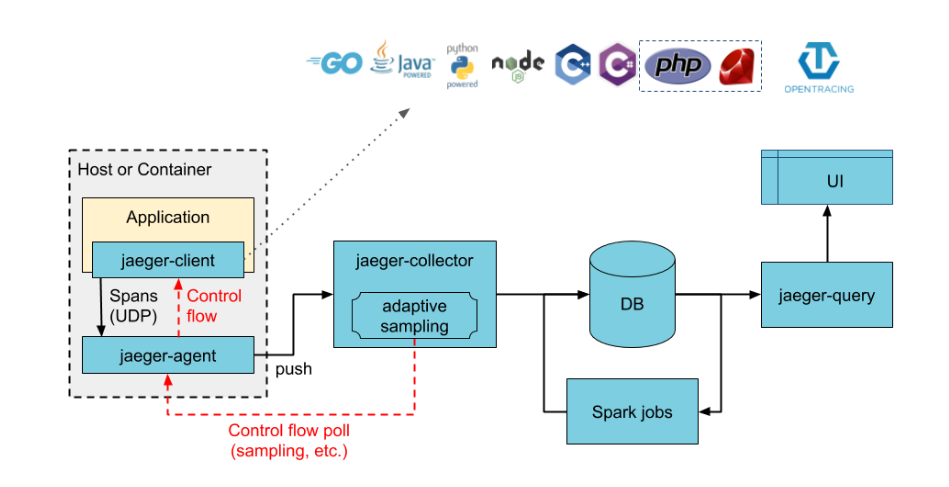
\includegraphics[scale=0.4]{32.png}
    \centering
    \caption{Schema logico dei componenti di Jaeger}
\end{figure}
I componenti possono essere avviati in container a sè stanti, oppure in un container all-in-on che li comprende tutti.\\
Di seguito possiamo vedere un' immagine dell'interfaccia grafica di jaeger.
\begin{figure}[H]
    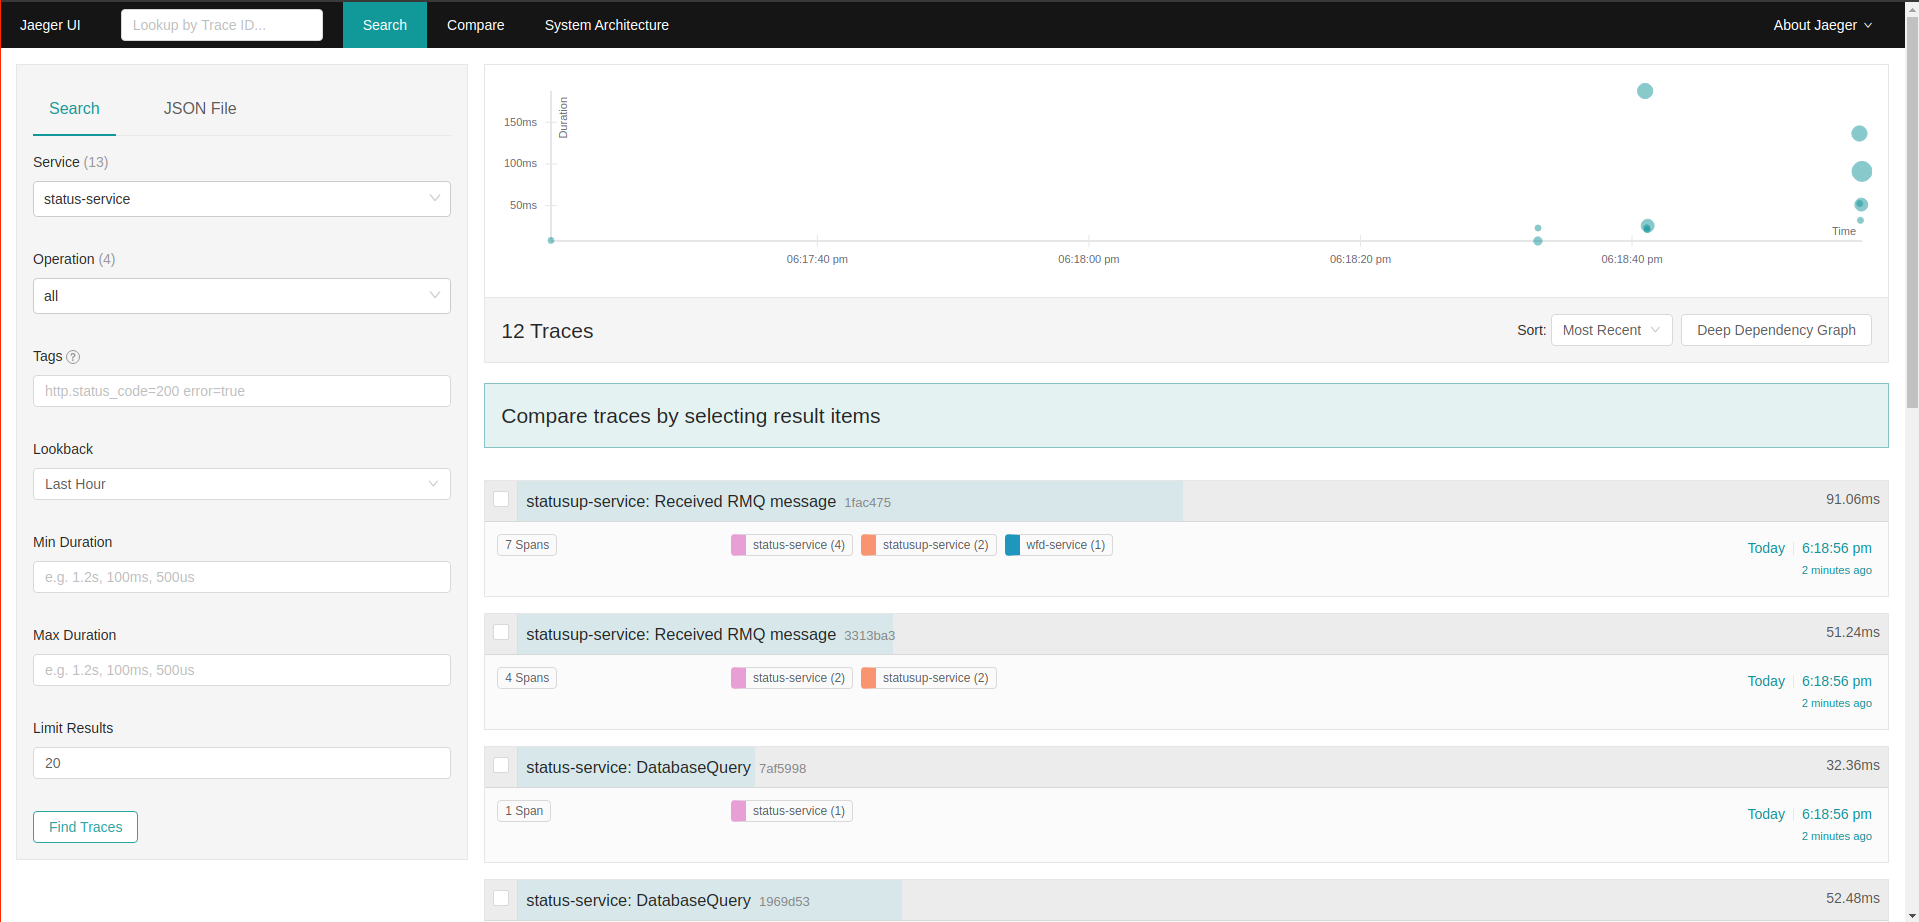
\includegraphics[scale=0.21]{48.png}
    \centering
    \caption{Interfaccia grafica dell' interfaccia Jaeger. In altro possiamo trovare un dashboard che rappresenta quali span sono stati registrati nel lasso temporale. A sinistra è possibile scegliere quale micro servizio tracciare, quale operazione e impostare i parametri di ricerca. Nella zona
    centrale/destra possiamo vedere l' elenco degli span registrati di quel micro servizio.}
    
\end{figure}

Inoltre, dopo aver registrato qualche span, jaeger si occupa anche di costruire un grafo che rappresenta quali micro servizi comunicano tra loro.

\begin{figure}[H]
    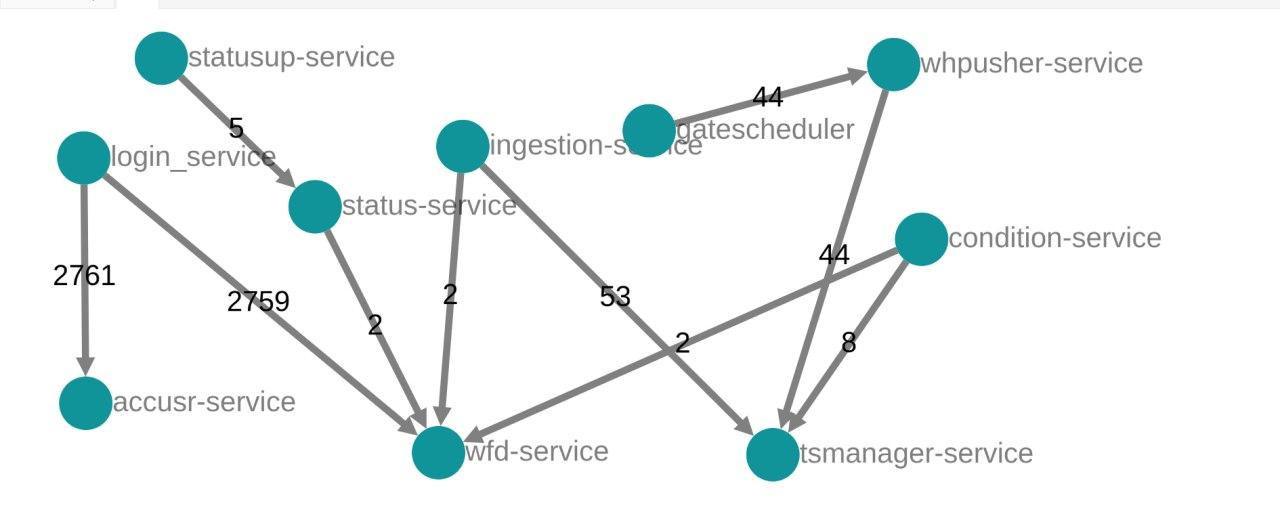
\includegraphics[scale=0.4]{grafo.jpg}
    \centering
    \caption{Grafo costruito automaticamente da Jaeger che costruisce tutti i collegamenti tra i vari servizi.}
\end{figure}

\section{Go kit}
Go kit\cite{go:2} è una libreria Golang che è stata utilizzata per lo sviluppo dello ZDM\cite{zdm:1}. Cercando tra la documentazione, sono stati trovati anche dei metodi relativi al tracing che si sono rivelati utili
per il tracing delle richieste HTTP tra i micro servizi. 
% TODO Cambia git in Gogs
\section{Gogs}
Gogs\cite{gogs:1} è una piattaforma che ospita un servizio di tipo git. Quindi similmente a Github facilita lo sviluppo di un software quando si è tante persone a svilupparlo. Lo zdm è stato sviluppato attraverso questa piattaforma, dunque è stato garantito l' accesso al tirocinante e si è creato un nuovo branch dove poter modificare il codice. 

\section{Docker}
Docker\cite{docker:1} è una piattaforma che permette di creare container (spazi virtuali) dove poter girare programmi in sicurezza, in modo tale che se tale programma presenta dei problemi non si riperquotono al di fuori del container. L' architettura dello ZDM\cite{zdm:1} prevede che ogni servizio giri nel proprio container; lo stesso si è deciso per Jaeger, dato che è un servizio esso stesso che comunica con i micro servizi.
\section{Easyredmine}
Easyredmine\cite{easyredmine:1} è una piattaforma online che rende più facile e intuitiva la gestione di lavoro degli sviluppatori di Zerynth, secondo le regole dello sviluppo AGILE.

\section{Rabbit Message Queue}
Rabbit Message Queue\cite{rabbit:1} (abbreviato RMQ) un protocollo di scambio di messaggi. Si basa sul concetto di pubblicare e prelevare messaggi su/da una coda di messaggi. Chi pubblica un messaggio non lo fa direttamente su una coda ma su un oggetto chiamato exchange. Ad un messaggio viene associato un \textit{topic}, ovvero un'etichetta per identificare l'argomento del messaggio. L'exchange si occupa di mettere quei messaggi nella coda giusta. Dall' altro lato chi 
vuole prelevare i messaggi di una coda deve sottoscriversi ad essa con un determinato topic. Allora verranno prelevati solo messaggi con il topic corrispondete a quello scelto durante la fase di iscrizione.\\
Qesto protocollo è stato usato attraverso la libreria GO amqp.
\section{Zerynth Device Manager}
Lo Zerynth Device Manager\cite{zdm:1} (abbreviato ZDM) l' applicazione distribuita di Zerynth. È un servizio per la gestione di device e di dati per registrare, organizzare, monitorare, aggiornare e gestire in maniera remota IoT device ( device dell' internet delle cose).
È anche l'applicazione su cui è dovuto implementare il sistema di tracing di micro servizi.

\chapter{Architettura generale del sistema di tracing}
In questo capitolo vedremo una descrizione quanto meno dettagliata dell' architettura del sistema. Si parlerà delle 3 principali comunicazioni tracciate, e per ognuna come si è realizzato il tracing attraverso le
tecnologie menzionate nel capitolo precedente.
\section{Main dei servizi e Client Jaeger}
Per prima cosa viene inizializzato il tracer nel main ( il file go principale del servizio). Questo tracer permette di creare gli span, viene settato come Tracer Globale attraverso il metodo della libreria di opentracing "setGlobalTracer()"; settandolo come tracer globale, si è in grado di accedervi in qualunque "zona" del codice del microservizio, e questo è fondamentale, in quanto ci permette di alleggerire
di molto il codice di ogni servizio, evitando di trascinare dietro il tracer. Per inizializzare il tracer si è creata una funzione che si occupa di settare le impostazioni corrette dello jaeger client e restituisce il nuovo tracer. Si è deciso di mettere le impostazioni
di Jaeger come variabili d'ambiente per ogni microservizio. Queste variabili d'ambiente servono per scegliere la configurazione dello jaeger client, in particolare del \textit{sampler}: il sampler è l' oggetto che definisce in che modo vengono mandati gli span allo jaeger collector. Ne esistono di più tipi, per ragioni di testing e debugging si è scelto un sampler probabilistico
 di parametro 1: un sampler che spedisce tutti gli span perché il parametro 1 equivale alla percentuale di span spediti (1=100\%). 
\begin{figure}[H]
    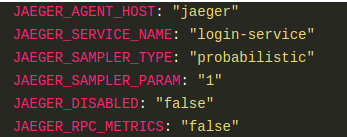
\includegraphics[scale=0.5]{envvar.png}
    \centering
    \caption{Variabili d' ambiente del servizio di login. Tra quelle obbligatorie si ha il nome del servizio e l' agent host, quest' ultimo è il nome dell'host dove risiede lo jaeger agent}
\end{figure}

Queste variabile d'ambiente vengono esportate in una struttura nel codice del main attraverso un metodo della libreria dello ZDM\cite{zdm:1} Utils, in particolare di un pacchetto chiamato "tracing" creato dal tirocinante.
\begin{figure}[H]
    \includegraphics[scale=0.5]{init.png}
    \centering
    \caption{Codice della funzione "init" che si occupa di inizializzare le varie configurazioni del servizio. L' ultima è la configurazione del client jaeger.}
\end{figure}
In questo pacchetto troviamo anche la funzione che restituisce il tracer menzionata prima.
Subito dopo aver creato il tracer si imposta come tracer globale, come spiegato qualche momento fa. Questo passaggio è molto importante perché si utilizzerà sempre il tracer globale,
dunque per evitare errori c'è bisogno che sia definito il prima possibile.
\begin{figure}[H]
    \centering
    \includegraphics[scale=0.5]{ini2.png}
    \caption{Esempio di codice che inizializza il tracer e lo imposta come global tracer.}
\end{figure}
\section{Tracing di richieste http}
Questo è il primo tipo di comunicazione di cui è stato sviluppato un sistema di tracing. Il concetto base per la propagazione di uno span tra due micro servizi è piuttosto banale: gli span vengono propagati tramite un contesto ( un oggetto del Golang), ovvero si può  creare un contesto e legare ad esso uno span. Quando viene eseguita una richiesta Http si può inserire negli header della richiesta il contesto contenente lo span. 
Dall'altra parte, quando si riceve una richiesta Http, basta estrarre dagli header il contesto contenente lo span e far partire un nuovo span figlio dello span del contesto. 
L'inserimento e l'estrazione di uno contesto in una richiesta Http è ottenuto attraverso i due metodi dell' oggetto tracer, tracer.Inject e tracer.Extract.
\subsection{Tracing del client Http}
Per il tracing dei servizi che fanno richieste Http ad un altro servizi, si è ampliato il pacchetto "micro", della libraria Utils dello ZDM\cite{zdm:1}, 
con dei nuovi metodi per arricchire il contenuto della richiesta con il contesto contenente uno span.
Nello ZDM\cite{zdm:1}, quando un servizio fa una richiesta Http si usa un oggetto chiamato "MicroCaller".
 Quest' oggetto (che fa parte del pacchetto micro) ha dei metodi per definire gli attributi della richiesta Http. Quello che si è fatto è stato semplicemente di aggiungere nuovi metodi per l'inserimento 
del contesto tra gli attributi della richiesta. Quindi per propagare il contesto tra due micro servizi basta utilizzare i nuovi metodi del pacchetto micro.
\subsection{Tracing del server Http}
Il discorso è un po' più complicato per i servizi che si comportano come server, ovvero quelli che ricevono le richieste Http. 
Ogni servizio "server" crea nel suo main un HttpServerHandler: un oggetto che si mette in ascolto su una determinata porta 
( definita dalle variabili d'ambiente) per servire le richieste Http. Quando viene creato quest'oggetto viene invocata una 
funzione che lo inizializza secondo determinate opzioni; una in particolare è stata utilizzata per estrarre il contesto dalla richiesta Http: le opzioni ServerBefore.
 Come si può intuire dal nome, sono una lista di funzioni che vengono eseguite prima del consumo della richiesta http, quindi appena
  arriva la richiesta il server esegue le funzioni contenute nelle opzioni ServerBefore. Tra queste funzioni
   si è inserita una funzione della libreria Go kit tracing, chiamta HTTPToContext; quello che fa è proprio estrarre il contesto
    della richieste e passarlo alla funzione successiva nella catena di chiamate. In questo modo  lo span è nel contesto di tutta
     la catena di chiamate che vengono eseguite.
Dopo di questo, il server chiama il metodo per gestire la richiesta ricevuta,in base al tipo di richiesta. In particolare per ogni tipo di richiesta viene creato un endpoint,
ovvero il "luogo" dove vengono gestite quel tipo di richiesta. Per tracciare l'operazione gestita dall'
endpoint si chiama una funzione della libreria Go kit tracing (la stessa libreria menzionata prima), la funzione in questione si chiama TraceServer; questo metodo prende due argomenti, il tracer (questo è il tracer globale) e il nome dell' operazione (il nome dell' operazione gestita dall' endpoint) e restituisce un nuovo endpoint, che però ha nel contesto un nuovo span creato dalla funzione stessa. Questo span sarà proprio il figlio dello span ricevuto nel contesto della richiesta Http. 

\section{Tracing di scambio di messaggi RMQ}
Il secondo tipo di comunicazione che si è tracciato sono lo scambio di messaggi Rabbit Message Queue. Il protocollo prevede un publisher e un subscriber, il publisher pubblica i messi su un oggetto chiamato exchange che smista i messaggi nelle code al quale è connesso. I messaggi vengono smistati in base al loro interesse, chiamato "topic". Il subscriber si può sottoscrivere ad una coda specificando il topic a cui è interessato. Quando nella coda è presenta un messaggio con quel topic, il subscriber viene avvisato e preleva il messaggio. I messaggi si chiamano delivery e possiedono diversi attributi,tra i quali degli headers simili a quelli delle richieste Http.
Il tracing di questo scambio è stato possibile grazie alla libreria amqptracer, che contiene i metodi per inserire ed estrarre il contesto dal messaggio nei e dai suoi header.
\subsection{Tracing del Publisher}
Ogni qual volta che un servizio vuole pubblicare un messaggio su una coda, dopo aver configurato il publisher nel suo main, deve chiamare il metodo "publish" del publisher. A questo metodo va passato un delivery che verrà pubblicato sulla coda ( impostata con l'inizializzazione del publisher). Per rendere possibile la propagazione del contesto, si è aggiunto a questo metodo un nuovo argomento oltre al messaggio: un contesto. In questo modo il metodo publish, prima di pubblicare il messaggio sulla coda, inserisce negli headers del messaggio lo span contenuto nel contesto passato al metodo publish.
L' inserimento del contesto (che in questo caso è uno spanContext e non un contesto vero e proprio) viene fatto attraverso una funzione della libreria amqptracer, amqptracer.Inject, che prende uno span e un delivery, e inserisce lo spanContext nel delivery.
\subsection{Tracing del Subscriber}
Per il tracing del subscriber si è aggiunta una funzione al pacchetto "queue" delle Utils dello ZDM\cite{zdm:1}. Questa funzione prende come argomento la funzione che si occupa del consumo del messaggio, la handleFunc:
in questo modo crea uno span prima del consumo del messaggio, lo inserisce nel messaggio e poi chiama la handleFunc e infine termina lo span. Questo procedimento viene fatto nella funzione ConsumeLoop del subscriber, ovvero il codice che si mette in ascolto di nuovi messaggi nella coda.
\\Oltre a questo meccanismo, similmente come per il tracing dei server Http, bisogna impostare tra le opzioni ServerBefore ( in questo caso sono le funzioni che vengono eseguite prima della ricezione di un messaggio) una funzione creata dal tirocinante; questa funzione non fa altro che creare uno span partendo dal contesto presente nel messaggio, ed inserirlo nella catena di funzioni che si 
occupano del consumo del messaggio. Anche in questo caso viene poi creato l' endopoint,  e si utilizza una funzione per impostare il nome dello span in base all' operazione gestita dall' endpoint.

\newpage

\section{Tracing di richieste ai Database}
Per il tracing di richieste ai Database si è aggiunto dei metodi nel pacchetto "db" (database) delle Utils dello ZDM\cite{zdm:1}. Se la variabile 
d' ambiente DB-TRACING è impostata a true allora viene eseguito il tracing altrimenti no(il valore di default è "true", dunque anche se 
non si specifica la variabile il tracing verrà effettuato).
In particolare, se la variabile d'ambiente è impostata a true, allora si aggiunge un "QueryHook" database. Questo QueryHook
 implementa due metodi, un before e  un after query. Questi metodi vengono chiamati prima e dopo dell'esecuzione effettiva della richiesta. L'implementazione della BeforeQuery prevede la creazione di uno span che poi viene terminato nella AfterQuery.
A livello di servizio, bisogna passare il contesto che si vuole tracciare alla richiesta al database. Per esempio, se un servizio volesse ottenere i dati di un utente attraverso un metodo che è del tipo "db.Select("query") bisognera usare un metodo alternativo del tipo "db.SelectWithContext(ctx,"query"), in modo da propagare il contesto (e lo span eventualmente presente nel contesto) attraverso la richiesta al database.


\newpage
\chapter{Lavoro svolto}
Le prime due settimane del tirocinio sono state di preparazione. Dopo essersi recati in ufficio per incontrare i tutori aziendali, si è discusso
del lavoro da fare e come farlo; si è introdotto il tirocinante nell'ambiente lavorativo e gli si è spiegato come lavorano.\\
Zerynth ha scelto, da qualche anno, il protocollo di sviluppo AGILE: lavorano in sprint di 2 settimane, ovvero: all'inizio dello sprint (o alla fine del precedente) programmano i propri "task" da svolgere per lo sprint; un task può essere un qualunque tipo di lavoro, che viene stimato da chi se ne occupa in un quantitativo di ore. Quindi si cerca di finire quel task nel tempo stimato, riportando giornalmente sulla piattaforma di Easyredmine quanto tempo si è lavorato a quel task.
Non finire un task nel tempo stimato non è necessariamente un problema; infatti questa stima è solamente una stima ottimistica. Inoltre ogni task ha una priorità ed è specificato se un task è "rimandabile", nel senso che si può rimandare allo sprint successivo, oppure "non rimandabile", ovvero un task con assoluta urgenza. Inoltre, secondo il metodo di sviluppo agile,  si lavora per raggiungere una \textit{"milestone"}, ovvero un obbiettivo da completare entro un determinato numero di sprint. Per esempio il sistema di tracing sviluppato da questo tirocinio è stato inserito proprio nel milestone più  vicino.\\
Quindi ci si è adattati a questo tipo di lavoro; si è inserito il tirocinante nella piattaforma e si è iniziato ad assegnargli task.\\
Da ora in poi questo capitolo sarà diviso in sezioni, dove ogni sezione corrisponde ad uno sprint di due settimane.
\\Questo capitolo è stato scritto come una specie di "diario" del lavoro svolto, quindi descrive sistema sviluppato da zero, dunque ci sono delle divergenze con l'architettura descritta nel capitolo 4, poichè quella è il risultato finale del sistema implementato, mentre in questo capitolo viene descritto il sistema durante la sua evoluzione.
\section{Primo sprint}

Nel primo sprint si è provveduto a preparare l'ambiente di lavoro sul PC del tirocinante, ovvero con l'aiuto del responsabile dello sviluppo software si è installato lo ZDM\cite{zdm:1}. Dopo di che si è passato a svolgere il primo task: studiare il progetto di opentracing, in particolare
si è seguito un tutorial sviluppato da uno dei creatori del progetto. Dopo aver preso dimestichezza con il progetto di opentracing, si è imparato i rudimenti del Go kit e capito come funzionano i micro servizi dello ZDM che usano questa libreria.
In seguito al completamento di questi due task, si è passato ad un primo approccio di tracing dello ZDM.
Insieme al supervisore si è studiato lo schema delle interazioni dei micro servizi dello ZDM\cite{zdm:1} per decidere su quali micro servizi iniziare lo sviluppo del sistema di tracing.
Alla fine di questo sprint (come in ogni sprint) si è tenuto lo sprint review, nel quale si è discusso insieme agli altri colleghi quali compiti si è  riuscito a fare e in quali si sono riscontrati problemi; dopo questa fase di revisione, si è passati al planning del nuovo sprint, ovvero si è deciso i nuovi task da assegnare ad ogni sviluppatore (compreso il tirocinante).
\begin{figure}[H]
    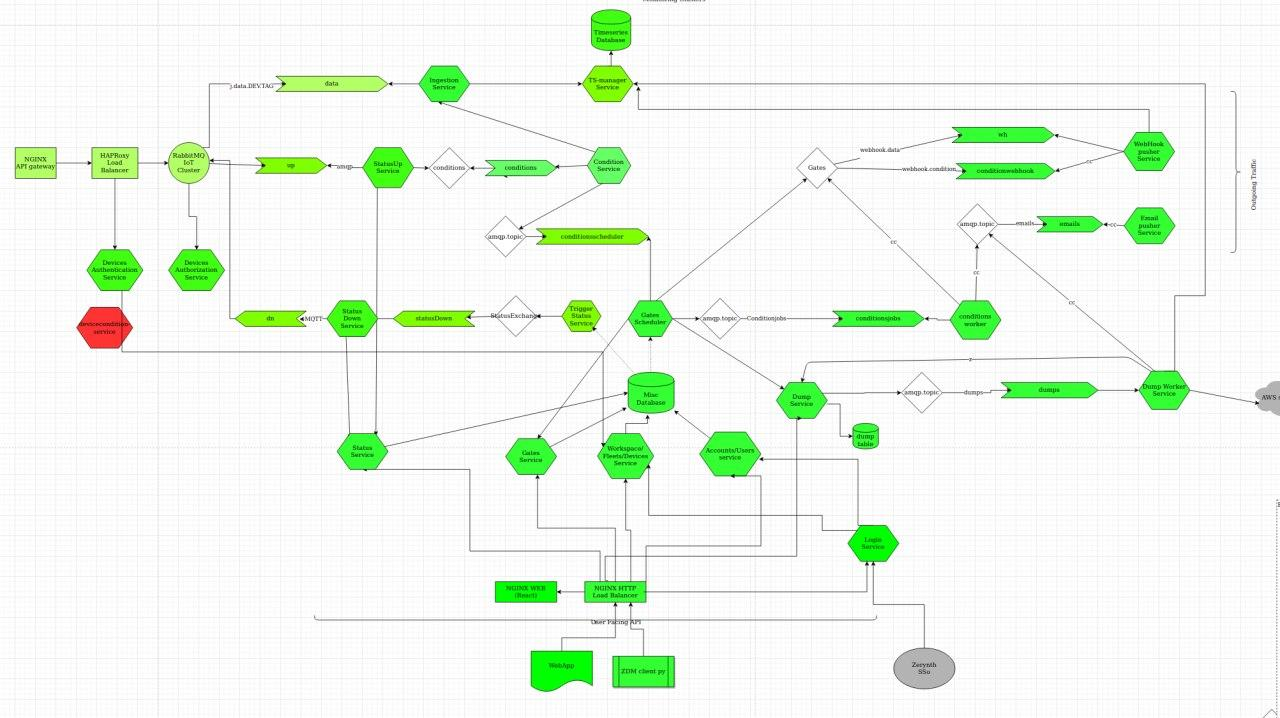
\includegraphics[scale=0.4]{41.jpg}
    \centering
    \caption{Schema logico dei micro dello servizi dello ZDM\cite{zdm:1}. Ogni esagono corrisponde ad un servizio, che sono collegati con i servizi con cui comunicano. Le frecce verdi "allungate" sono code di messaggi, collegate ai servizi che prendono i messaggi e che li pubblicano sulla coda }
\end{figure}  

\newpage
\section{Secondo sprint}
In questo sprint si è realizzata la prima implementazione del tracing di richieste Http e scambi di messaggi RMQ. Prima si 
è sviluppato il codice per l'inizializzazione del tracer e della configurazione dello jaeger client. Poi si discute del tracing delle comunicazione di alcuni microservizi.



\subsection{Impostazioni del client Jaeger}
Il modo in cui vengono mostrati gli span nella GUI di Jaeger dipende esclusivamente dalla configurazione del client jaeger.
La configurazione è una struttura chiave valore che imposta i paramatri del client; i parametri usati per una prima implementazione sono stati il nome del servizio (obbligatorio), l' host del servizio jaeger (obbligatorio) e poi il tipo di \textit{sampler}. Il sampler è l' oggetto che determina come verranno mandati gli span allo jaeger collector:
ci sono più tipo di sampler ad esempio si ha il \textit{costant} sampler, che manda tutti gli span registrati; oppure il \textit{probabilistic} sampler che prende come parametro un numero tra 0 e 1 che rappresenta la probabilità che quello span venga mandato al collector. Questa differenziazione è presente perché gli span registrati in un' architettura a micro servizi possono essere molti, anche migliaia. Essendo in una fase di sviluppo conviene però monitorare tutti gli span registrati dal client, dunque un sampler di tipo costante fa al caso nostro.
Tutte queste impostazioni sono ottenute attraverso delle variabili d' ambiente.
\\ Di seguito possiamo vedere il codice della funzione che inizializza il tracer con la configurazione dello jaeger client presa dalle variabili d 'ambiente.
Il tipo di sampler usato è costante, poichè è stato necessario in fase di testing vedere ogni span registrato, a fini di debugging.
\begin{figure}[H]
    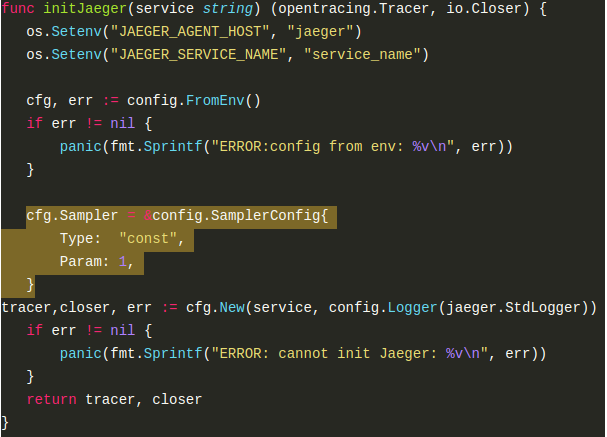
\includegraphics[scale=0.5]{92.png}
    \centering
    \caption{Prima implementazione del metodo che crea un tracer secondo i parametri del client jaeger}
\end{figure}  
Questa implementazione verrà poi cambiata nella build finale del sistema, come vedremo nella sezione dedicata al refactoring nell' ultimo sprint.
\subsection{Tracing di richieste HTTP}
%TODO migliorare descrizione architettura richieste http
Si è deciso che i primi micro servizi da tracciare fossero il login-service, l'accusr-service e wfd-service. Le operazioni coperte da questo trace sono quelle iniziali, ovvero di login, ottenimento dell'account dell'utente e del suo spazio di lavoro.
Essendo il primo trace realizzato per lo ZDM\cite{zdm:1} si è proceduto per gradi. Come prima cosa si è capito che tipo di comunicazione fosse: una richiesta da parte del login service al accusr e wfd service tramite HTTP;
opentracing prevede un tracciamento di questo tipo attraverso gli header della richiesta http: gli span del login service che rappresentano le richieste agli altri due micro servizi vengono inseriti nell' header HTTP sotto forma di mappa chiave valore.
Dall'altra parte i micro servizi che ricevono la chiamata riescono a estrarre dagli header della richiesta il contesto dello span, e dunque creare un nuovo span figlio di esso per ottenere una continuità tra le chiamate e costruire una specie di albero di richieste.
Dopo una prima implementazione "hardcodata"\footnote[1]{Quando un codice è scritto in modo brutto, per vedere se funziona} , scrivendo il codice per una grezza richiesta http nello ZDM\cite{zdm:1} e verificando che funzioni correttamente si è passato poi a creare una versione universale per tutte le richieste HTTP, modificando la librearia dello ZDM\cite{zdm:1} chiamata "Utils" che si occupa dello scambio di messaggi HTTP.
\begin{figure}[H]
    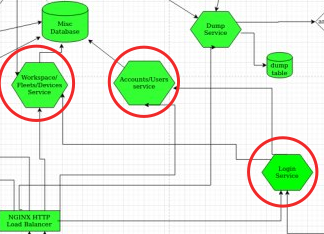
\includegraphics[]{42.png}
    \centering
    \caption{Login, accusr, wfd service nello schema}
\end{figure}

\begin{figure}[H]
    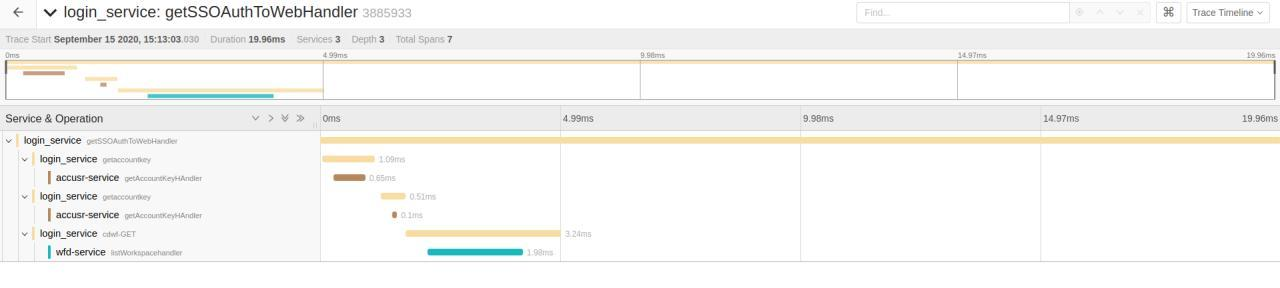
\includegraphics[scale = 0.4]{43.jpg}
    \centering
    \caption{Risultato del primo trace sviluppato nei 3 servizi di login,accusr e wfd}
\end{figure}
Nelle due figure precedenti si può vedere la comuniazione di quei 3 servizi. Il login service riceve richieste direttaente dalla webapp dello ZDM\cite{zdm:1} dunque è la radice della comunicazione. I servizi accusr e wdf (worker device fleet) sono invocati dal login service e si occupano di fornire al medesimo i dati dell' utente (accusr) e lo spazio di lavoro e di device registrati (wfd).
\subsection{Tracing di scambio di messaggi RMQ}
Dopo aver realizzato un modo per tracciare le richieste HTTP dei micro servizi, qualunque sia il micro servizio attraverso l'implementazione nella libreria di supporto, si è passato al task di implementare
il tracing di un altro tipo di comunicazione: lo scambio di messaggi attraverso il protocollo Rabbit MSQ (vedi CAP. 3 Tecnologie utilizzate).\\
In questo caso un micro servizio che vuole pubblicare un messaggio su una coda (sono quelle frecce verdi allungate nella figura 5.1) deve pubblicare i messaggi sull'exchange della coda (i rombi bianchi nella figura 5.1). Dunque bisogna  inserire il contesto dello span che rappresenta la pubblicazione del messaggio nel messaggio stesso. Questo è stato effettuato tramite una libreari di supporto amqptracer; ogni messaggio, similmente ad una richiesta htpp, possiede degli headers; la libreria di supporto permette di inserire il contesto negli headers e dall'altra parte, quando un servizio preleva un messaggio, estrarre il contesto per creare uno span figlio di quello nel contesto.
Per far ciò si è direttamente implementato il sistema nella libreria menzionata prima, le "Utils". Infatti questa libreria permette ai micro servizi di pubblicare messaggi e sottoscriversi alla ricezione dei messaggi dalle code.\\
Questo sistema è stato prima testato sui micro servizi triggerstatus e statusdown.
\begin{figure}[H]
    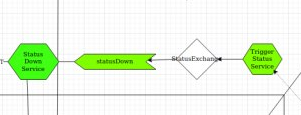
\includegraphics[]{44.png}
    \centering
    \caption{triggerstatus, statusdown, exchange e coda di messaggi interessata}
\end{figure} 

\begin{figure}[H]
    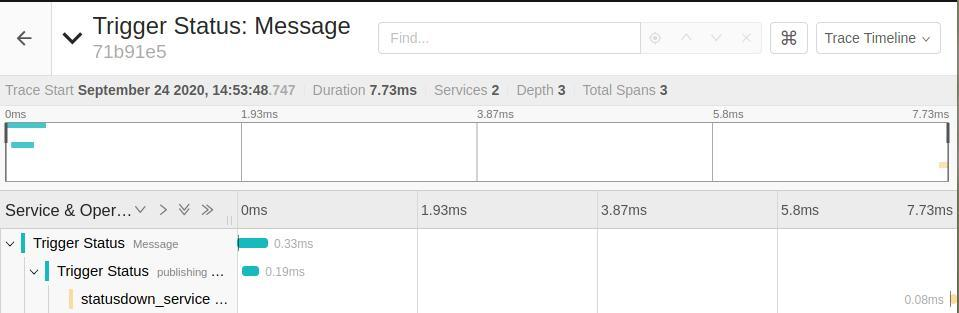
\includegraphics[scale=0.5]{45.jpg}
    \centering
    \caption{Risultato del traci di un messaggio RMQ nella GUI jaeger}
\end{figure}
Come si puó vedere nella figura 5.6, il trace di un messaggio rmq appare un po' diverso: lo span del servizio che legge il messaggio (statusdown service) non appare sotto lo span di quello che lo ha pubblicato (triggerstatus service); appare dopo un gap di tempo, come è giusto che sia, dato che il messaggio viene pubblicato sull' exchange della coda, poi messo nella coda e infine letto dal servizio che se ne occupa.
La comunicazione tra triggerstatus e statusdown avviene quando veniva depositato un nuovo dato del database collegato al triggerstatus. Quando captava questo evento, il triggerstatus manda il messaggio rilevato del database allo statusdown.

\newpage
\section{Terzo sprint}
In questo sprint si è sviluppata la prima versione di tracing delle richieste ai database. Dopo di che si è implementato il sistema complessivo sviluppato finora (Http, RMQ, db) su altri microservizi che vedremo nel dettaglio.

\subsection{Tracing delle richieste ai database}
Come si è visto dalla figura 5.1, nello ZDM\cite{zdm:1} sono presenti diversi database che contengono i dati degli utenti, i dati spediti dai device connessi allo ZDM\cite{zdm:1} e così via; dunque il primo task per questo sprint è stato di 
tracciare le richieste dei micro servizi ai database. Questo è stato implementando modificando la libreria Utils, che si occupa di fornire ai servizi alcuni
 metodi per la gestione dei database; 
dunque si sono inseriti i metodi relativi al tracing in questa libreria, che sono stati poi usati negli micro 
servizi quando viene effettuata una chiamata a un database. Per ottenere ciò si è sfruttato un oggetto già usato dallo ZDM\cite{zdm:1}, il databaseLogger. Il databaseLogger si occupa di loggare tutte le chiamate fate a i database definendo due metodi: BeforeQuery e AfterQuery. 
Come si può intuire da nome, questi metodi vengono chiamati prima e dopo l' esecuzione di una query al database, dunque si è sfruttato questo meccanismo e inserito il codice di opentracing per creare span in questi due metodi.
Il risultato ottenuto è stato quello di poter visualizzare gli span che rappresentano una richiesta ai database tra gli span delle richieste http e richieste di messaggi; di seguito un esempio.
%TODO inserire figura database quuery
\begin{figure}[H]
    \includegraphics[scale=0.21]{database.png}
    \centering
    \caption{Risultato delle richieste ai database nella GUI jaeger}
\end{figure}

\subsection{Implementazione del tracing per altri micro servizi}
Dopo aver affinato l' implementazione di  opentracing per i 3 tipi di comunicazione dei micro servizi dello ZDM\cite{zdm:1}, si è passati ad estenderla a ad altri micro servizi;
le operazione che si sono tracciate in questa fase sono relative allo scambio dei dati dei device connessi allo ZDM\cite{zdm:1} tra i micro servizi; tutta questa operazione è una combinazione di richieste HTTP, scambio di messaggi RMQ e richieste ai database. Quindi senza entrare troppo nei dettagli ecco alcune immagini esplicative delle interazioni e dei risultati ottenuti.\\
Di seguito riporto la stessa immagine dello schema logico delle interazioni dello ZDM\cite{zdm:1}, nel quale si è evidenziato quali servizi si sono tracciati.
\begin{figure}[H]
    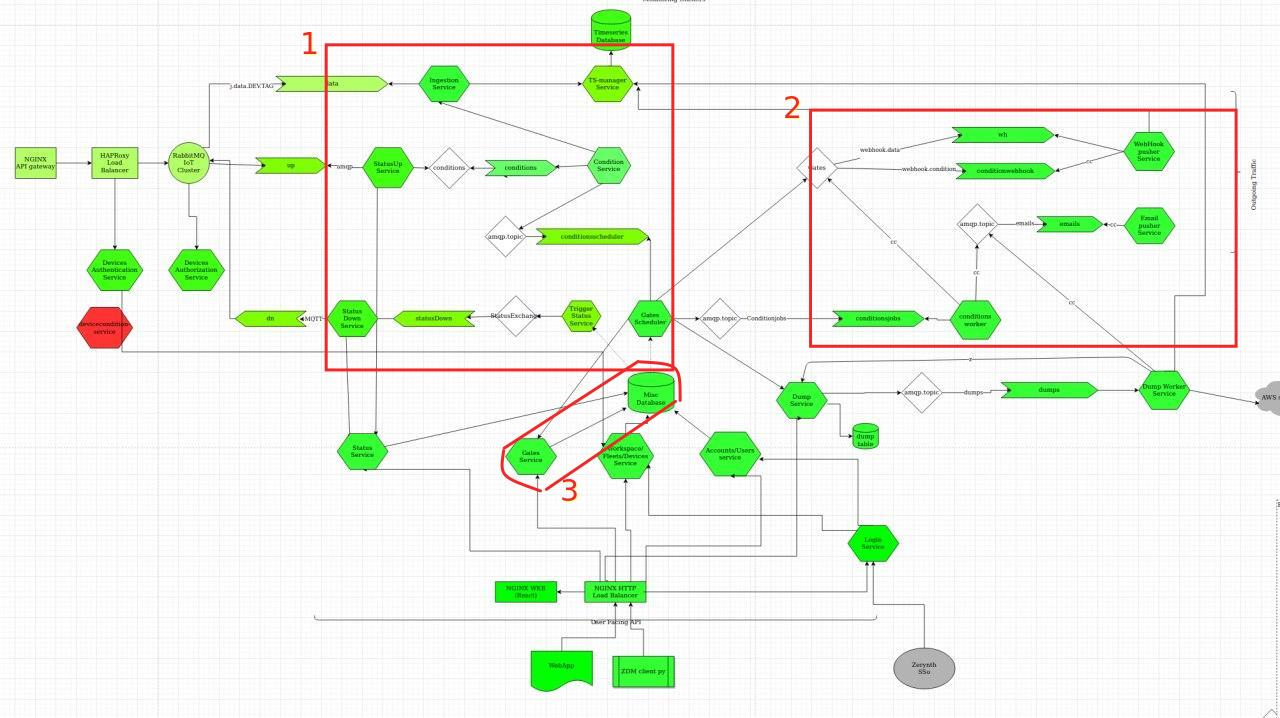
\includegraphics[scale=0.3]{61.jpg}
    \centering
    \caption{1.Interazioni tra i servizi di status, tsmanager, ingestion, condition, gatescheduler 2. Interazioni tra conditionworker,whpusher,emailpusher 3 interazione tra gate service e database}
\end{figure}

Avendo a questo punto già sviluppato le librerie e le migliori pratiche per tracciare le comunicazioni dello ZDM\cite{zdm:1}, quello che è bastato fare è stato applicare quello che è già stato applicato per gli esempi dello sprint precedente.
\\ La difficoltà si è spostata dal capire come implementare in modo generale il tracing a una comunicazione tra micro servizi, a dover usare quello che si è sviluppato su tutti i micro servi che ancora non sono stati tracciati.\\
In merito alla figura 4.7, si farà riferimento ad ogni riquadro e si descriverà brevemente quali tipi di comunicazioni avvengono tra i micro servizi interessati.

\subsection{Riquadro 1}
Queste comunicazioni nascono quando un device collegato allo ZDM\cite{zdm:1} invia dei dati a quest'ultimo; i servizi che per primi ricevono questi dati
 sono l' ingestion-service e lo statusup-service, in particolare li ricevono prelevandoli dalle code di messaggi a cui sono collegati, quindi qui si è 
 trattato di tracciare uno scambio di messaggi RMQ. L' ingestion service, dopo aver elaborato il dato ricevuto, lo manda al tsmanager tramite
richiesta HTTP. Lo statusup-service invece manda il suo elaborato tramite RMQ al condition-service e fa anche una richiesta http allo status service. 
Quest' ultimo in seguito a questa richiesta, esegue una database query; questa database query fa scattare il triggerstatus-service, che scrive sulla coda che
 comunica con lo statusdown-service questo avvenimento (questa è la comunicazione usata per testare il tracing RMQ). In parallelo, il condition service manda il messaggio ricevuto dallo statusup al gatescheduler service, che si occuperà infine di passare il messaggio nell'altro riquadro. Come potete notare, spiegare tutte queste interazioni è molto confusionario, ed è qui che entra in gioco il lavoro svolto durante questo tirocinio. Di seguito delle immagini che traducono tutto quello che è stato appena spiegato.
\begin{figure}[H]
    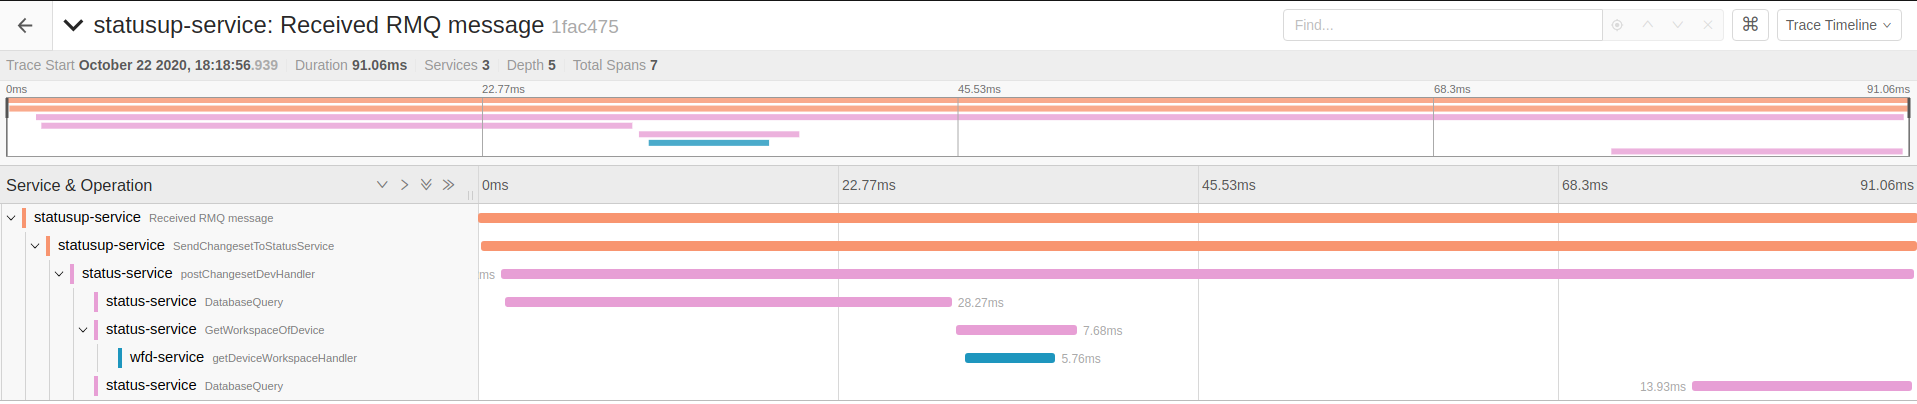
\includegraphics[scale=0.21]{49.png}
    \centering
    \caption{statusup,status, database, wfd service}
    
\end{figure}
\begin{figure}[H]
    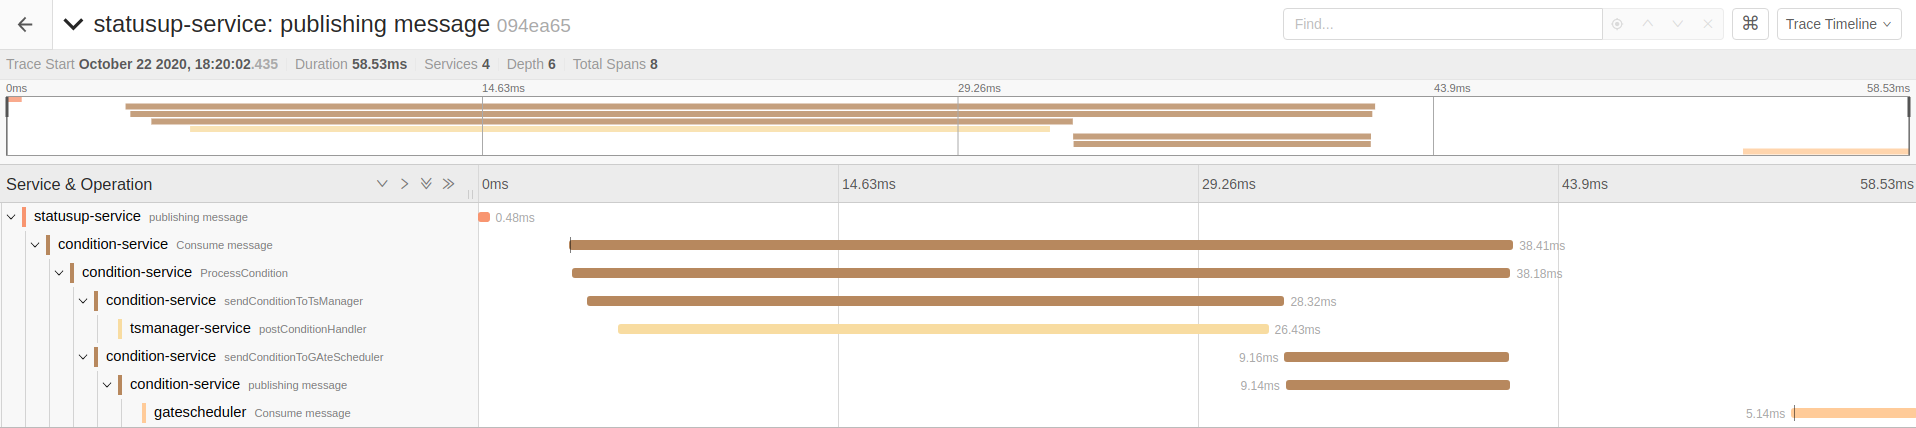
\includegraphics[scale=0.21]{51.png}
    \centering
    \caption{statusup,condition, tsamanager, gatescheduler service}
    
\end{figure}

\begin{figure}[H]
    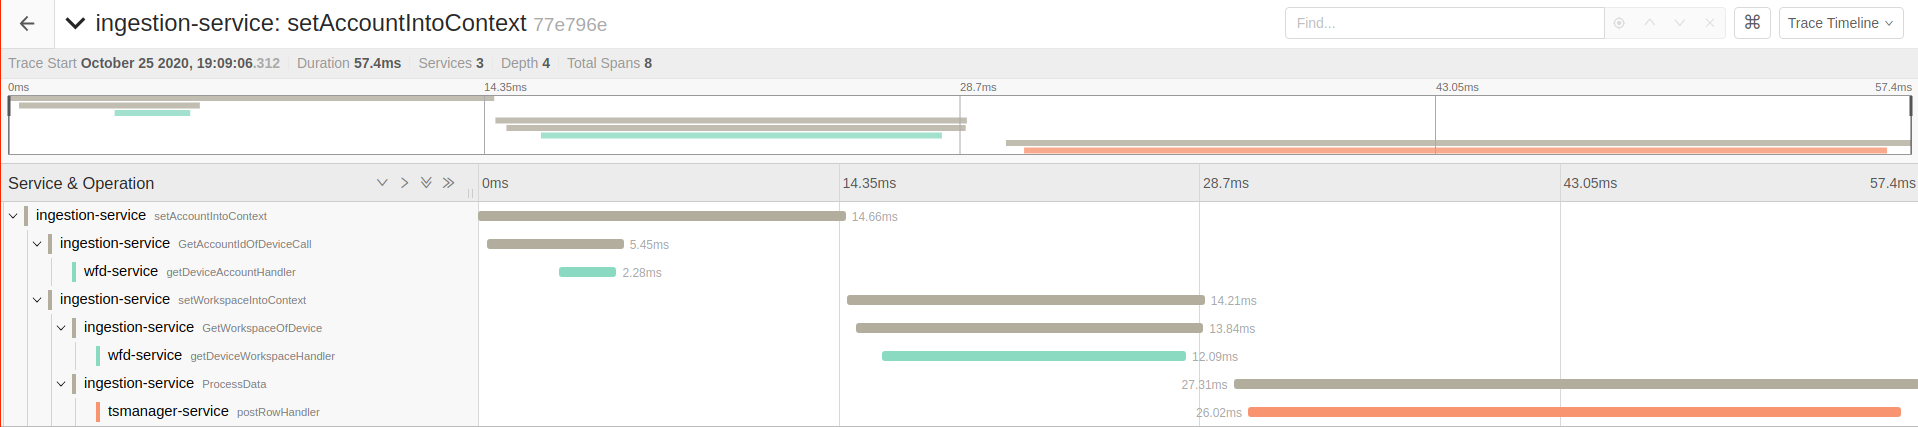
\includegraphics[scale=0.21]{75.png}
    \centering
    \caption{Trace della comunicazione tra ingestion service,wfd service e tsmanager service. Avviene quando un device manda un messaggio per ottenere l'account e lo spazio di lavoro dell' utente.}
\end{figure}
\subsection{Riquadro 2}
Ora le comunicazioni del riquadro numero 2. Dopo che il gatescheduler riceve i dati dai device, li smista in due code diverse: una per i dati di tipo "\textit{data}" e una per i dati di tipo "\textit{condition}". I primi vengono poi prelevati dal whpusher-service (webhook), i secondi anche dal conditionworker-service se è stato settato un  allarme per alcuni dati. Il whpusher poi fa una richiesta al tsamanager, il condition worker invece manda i dati all' emailpusher-service, che si occupa di avvisare l'utente tramite email di alcuni dati che rispettano una certa condizione.
\\Durante il lavoro si è distinto questi due flussi come il data flow e il condition flow. Di seguito delle immagini che raffigurano il risultato ottenuto.

\begin{figure}[H]
    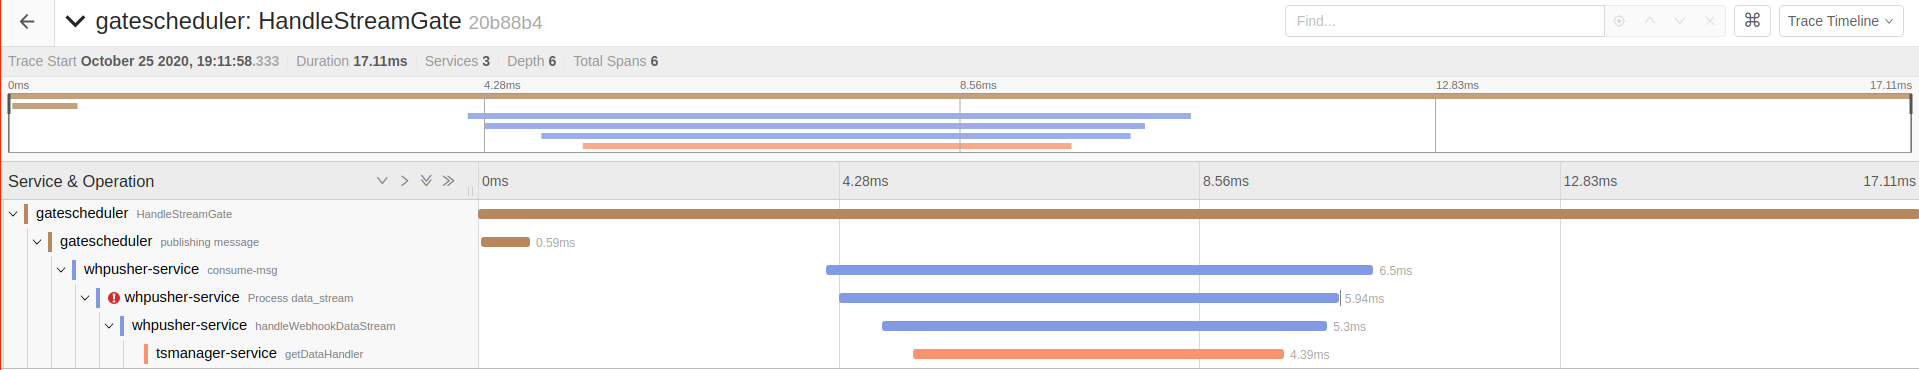
\includegraphics[scale=0.21]{76.png}
    \centering
    \caption{Trace del data flow}
\end{figure}
\begin{figure}[H]
    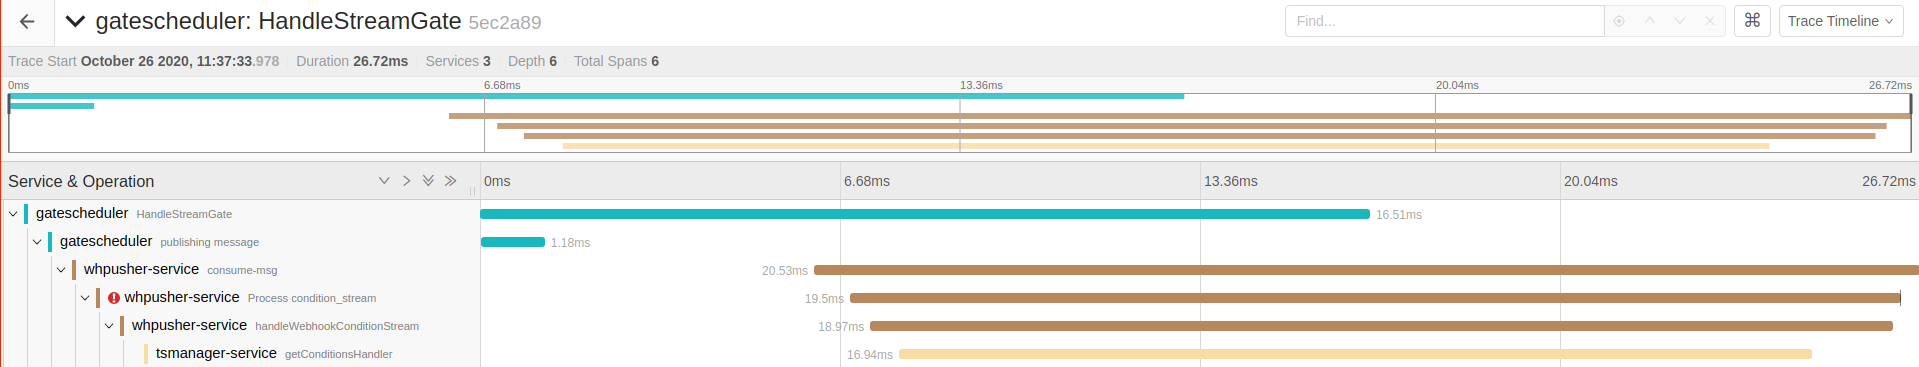
\includegraphics[scale=0.21]{77.png}
    \centering
    \caption{Trace del condition flow}
\end{figure}
\begin{figure}[H]
    \includegraphics[scale=0.21]{email.png}
    \centering
    \caption{Trace del percoso che fa un dato che viola una certa condizione (impostata da webapp), fino alla comunicazione per emil dell' emailpusher}
\end{figure}

\subsection{Riquadro 3}
Qui si è semplicemente tracciato tutte le comunicazione che esegue il gates service con il suo database. Di seguito un' immagine esplicativa.
\begin{figure}[H]
    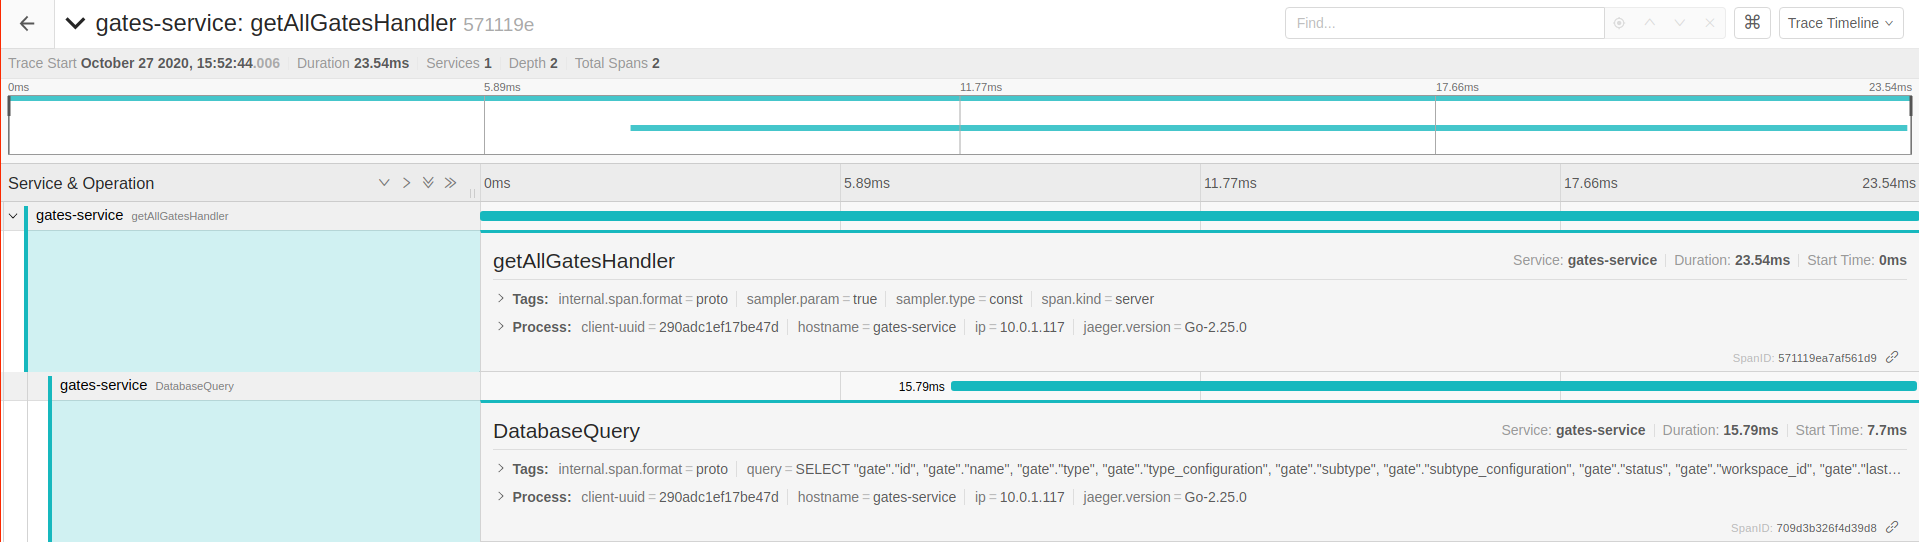
\includegraphics[scale=0.21]{90.png}
    \centering
    \caption{Esempio di richiesta database del gates service}
\end{figure}
\newpage
\section{Quarto sprint}
Questo è stato lo sprint finale; in questa fase si è occupati di rifinire un pò tutte le implementazioni di tracing. Si è partiti da un piccolo refactoring per aggiungere tutti i 
nuovi metodi alla libreria di supporto Utils dello ZDM\cite{zdm:1}.\\
Poi si è passato alla stesura della documentazione relativa all' architettura dell'implementazione.\\Si è conclusa con la fase di testing per il deployment del sistema e conclusione del tirocinio.


\subsection{Refactoring}
Questo task riguardava la rifinitura di alcuni punti lasciati in sospeso del sistema di implementazione, ad esempio includere nelle librerie dello ZDM\cite{zdm:1} alcuni metodi per l'inizializzazione del client jaeger, il settaggio di tutte le variabili d' ambiente di tutti i micro servizi relativi alla configurazione di jaeger.
Insomma una specie di revisione del lavoro svolto fin'ora.
Prima di tutto si è scritta una libreria apposita per tutti i metodi relativi al tracing; questa libreria, chiamata semplicemente "tracing", 
è stata inserita nella librearia "Utils" dello ZDM\cite{zdm:1}.
Prevede principalmente i metodi per creare un nuovo tracer con le impostazioni del client jaeger prese dalle variabili d' ambiente.
Poi si è anche effettuato un refactoring del tracing dello scambio di messaggi RMQ; infatti si è reso più simile a quello delle
 richieste Http per quanto riguarda i subscriber: quando un subscriber si registra, adesso deve definire un proprio "server" che è in ascolto sui messaggi.\\
Esattamente come per i server delle richieste http (4.4.2) si
è creata una funzione da inserire nelle opzioni "ServerBefore" che estrae il contesto contenuto nel messaggio (il delivery)
 e lo inserisce nel contesto passato alla catena di funzioni che si occupano del messaggio.
 \\Infine si è effettuato un refactoring del tracing delle richieste ai database. Come il lettore può ricordare dal capitolo 5 sezione 5.3.1, il tracing delle richieste database avveniva attacondosi alla struture del DatabaseLogger. Il problema è che 
 questa struttura serve esclusivamente per il logging delle query effettuate e non del tracing, dunque usarlo per ambo gli scopi (tracing e logging) non è una scelta giusta. Anche perchè il logging delle richieste ai database sono lunghi e sporcano molto il log del servizio rendendo più macchinoso trovare un eventuale errore.
 Dunque si è creata una struttura a parte, un nuovo QueryHook chiamato (con molta fantasia) DatabaseTracer; anch'essa implementa i due metodi after e before query, e in questo modo si è separato il meccanismo di tracing e quello di logging.
 
 \subsection{Documentazione}
 La prima cosa presa in considerazione per scrivere la documentazione è stata  a chi fosse rivolta. La documentazione è ai programmatori che devono estendere il servizio di tracing a nuovi micro servizi. Come sappiamo un architettura a micro servizi è molto dinamica, il che è sia un vantaggio che non. Difatti l' applicazione puó crescere aggiungendo micro servizi e se si aggiunge un micro servizio bisogna anche implementare il sistema di tracing su quel micro servizio.
 Dunque la documentazione è stata scritta con questo presupposto, ovvero pensata per i programmatori che dovranno tracciare nuovi micro servizi o anche modificare il tracing di quelli gia tracciati.\\
 La prima parte riguarda l'architettura generale del sistema, le librerie utilizzate e le migliori pratiche da utilizzare. Poi si passa a spiegare in particolare come tracciare i 3 tipi di comunicazione dello ZDM\cite{zdm:1}, ovvero richieste HTTP, messaggi RMQ e richieste ai database. 
 Infine una breve guida su come creare nuovi trace e span senza dover per forza utilizzare i metodi messi a disposizione dal sistema sviluppato dal tirocinante. 


\subsection{Testing}
Per la fase di testing si è eseguito il deployment dei servizi tracciati in questo tirocinio sulla versione di test dello ZDM\cite{zdm:1}.
 Da questa versione dello ZDM\cite{zdm:1} si sono eseguiti dei test per verificare il corretto funzionamento delle funzioni aggiunte al codice.\\
Prima del deployment, però , si è dovuto testare tutti i microservizi in locale, eseguendo per ognuno lo script che fa partire tutti i test Go;
 dopo aver sistemato i file di test Go ed essersi assicurati che tutti i servizi passassero tutti i test, si è potuto effettuare il deployment di questi servizi in testing.\\ 
Si sono però presentati alcuni intoppi: qualche servizio non riportava correttamente gli span. 
Dopo aver visto i file di log dei vari container dei servizi in testing si è subito notato che c'è stato un problema nel caricare la versione giusta di alcuni microserivi; dopo aver risolto questo piccolo difetto, il sistema sviluppato fino a questo momento funzionava senza problemi.
\\In questa fase non ci si è solo assicurati che il sistema funzioni correttamente ma ci si è anche domandato quali aspetti si potessero migliorare. Innanzi tutto , il supervisore ha fatto notare che alcuni trace erano superflui, quelli che riguardavano alcune query database che apparivano come singoli span, poiché erano richieste che partivano senza uno span radice, dunque apparivano come singoli span, i quali anche 
se potevano contenere informazioni utili, non avevano informazioni su quale matedo le ha invocate.
\cite{opentracing:1}
\chapter{Conclusione}
Icdn questo capitolo si tireranno le somme, si commenterà in generale il lavoro svolto, se è stato soddisfacente, se si è raggiunto l' obbiettivo del tirocinio e si discuteranno delle nuove skill acquisite dal tirocinante.
\section{Skill acquisite}
Tra la varie skill acquisite si riportano quelle più rilevanti.
\begin{itemize}
    \item[] \textbf{Git}: acquisita dimestichezza nell' uso dei comandi Git, e quindi anche di lavorare in un ambiente di sviluppo condiviso con più sviluppatori.
    \item[] \textbf{Sviluppo AGILE}: utilizzando i principi di questo metodo di lavoro , il tirocinante è riuscito ad adattarsi ad essi ed integrarsi nel flusso di lavoro dell'azienda, partecipando alle riunioni (sprint review) e discutendo del lavoro svolto e quello da completare.
    \item[] \textbf{Docker}: acquisita dimestichezza nell' uso di docker e docker compose.
    \item[] \textbf{Golang}: acquisita dimestichezza nell' uso di Golang e delle sue pratiche.
    \item[] \textbf{Architettura}: approfondito in modo pratico il funzionamento di un' architettura a micro servizi, solo accennata nei corsi di studio seguiti dal tirocinante.
    
\end{itemize}

\section{Commenti sull'Ambiente Lavorativo}
Sin dai primi contatti con l' azienda Zerynth / TOI srl il tirocinante ha subito avuto un impatto positivo. I miei supervisori si sono sempre dimostrati disponibili per ogni cosa.
I primi giorni il tirocinante di si è recato in persona in ufficio e lavorato lì, soprattuto per discutere di come implementare il sistema e preparare l'ambiente di sviluppo. Durante questo periodo è stato continuamente aiutato dai vari sviluppatori del team ZDM\cite{zdm:1} e messo a proprio agio.
Dopo questa fase iniziale, il lavoro si è spostato principalmente a casa del tirocinante per via dell' emergenza sanitaria, tuttavia queso non ha impattato troppo il lavoro svol. Al tirocinante è stato fornito modo di comunicare costantemente con il leader dello sviluppo software D. Neri, senza il quale questo progetto sarebbe stato molto più arduo da completare.
Come mezzi di comunicazione si è usato Telegram,Discord, Meet, Slack, strumenti molto familiari al tirocinante quindi non hanno presentato alcun problema. C'è comunque il bisogno di riportare che il lavoro da casa non è efficiente tanto quanto quello in un ambiente lavorativo come quello dell' ufficio dell'azienda, dove il tirocinante sarebbe stato stimolato molto di più e ricevuto un aiuto molto più immediato. 
\\ In ogni caso, l'esperienza lavorativa è stata senza dubbio positiva, e consiglierei ad un eventuale lettore in dubbio sul tirocinio, di optare per quest' azienda .


\section{Raggiungimento dell' obbiettivo e commenti sul lavoro svolto}
Un piccolo riassunto per fissare bene i concetti visti in questa relazione:\\
per prima cosa si è spiegato come si è iniziato a lavorare, la preparazione dell'ambiente di sviluppo, lo studio autonomo del linguaggio di programmazione 
Golang, le librerie di opentracing e jaeger, Gokit, Rabbit MQ. \\
Dopo le tencologie si è passati a descrivere l' architettura finale del sistema di tracing e il capitolo successivo riguarda invece il "come" è stato sviluppato. 
Quindi si è passati alla descrizione di come si è implementato il tracing
di richieste HTTP tra microservizi di tipo client / server. Poi il tracing dello scambio di messaggi delle ode RMQ. Infine  il tracing delle richieste ai database.
Dopo aver affinato queste implementazioni e inserite nelle librerie dello ZDM\cite{zdm:1}, si è passato ad implementarle in altri microservizi. Infine c'è stata una fase di testing e la stesura della documentazione.

L'autore del lavoro si ritiene abbastanza soddisfatto del risultato ottenuto, rispetta abbastanza gli obbiettivi presupposti dal tirocinio; tuttavia si poteva fare anche di meglio, e con più tempo a disposizione e una situazione lavorativa piú comoda sicuramente si sarebbe ottenuto un risultato migliore. 
Malgrado ció il tirocinante è fiducioso nel dire che il lavoro svolto ha portato ad un sistema, seppur non completo (alcuni servizi non sono stati tracciati, per mancanza di tempo o per altri motivi), funzionante ed utile agli sviluppatori dello ZDM\cite{zdm:1}.


\appendix
\bibliography{biblio}
\bibliographystyle{ieeetr}

 
\paragraph{Ringraziamenti}


\end{document}